\documentclass{article}

\usepackage[utf8]{inputenc}
\usepackage{graphicx}
\usepackage{listings}
\usepackage{indentfirst}  % <-- Add this line
\usepackage{hyperref} % Include this line in the preamble of your document
\usepackage{ulem} % Include this line in the preamble of your document


\title{
\Huge
Bsc Önálló Laboratórium

-

“Szabadítsd fel Bertalant! Szöveges válaszok automatikus kiértékelése nagy nyelvi modellel”

-

Dokumentáció
}

\author{\Large Konzulens: Dr. Forstner Bertalan\\
\Large Készítette: Fogti István HN4DTH fogtiistvan47@gmail.com\\}
\date{\today}

\makeatletter         
\def\@maketitle{
\newpage
 \null
 \vskip 2em%
 \begin{center}%
  {\Huge \@title \par}%
  \vskip 5em%   % <-- Modify this length to adjust the space
  {\large
   \lineskip .5em%
    \begin{tabular}[t]{c}%
     \@author
    \end{tabular}\par}%
  \vskip 1em%
  {\large \@date}%
 \end{center}%
 \par
 \vskip 1.5em}
\makeatother

\begin{document}

\maketitle
\thispagestyle{empty}
\newpage

\section{Téma Leírása}
Az oktatói lét egyik nehezen automatizálható feladata azoknak a kisZH vagy laborbeugró feladatoknak a javítása, amelyekre szöveges válasz érkezik. Nagy nyelvi modellek segítségével azonban előzetes vélemény mondható arról, hogy egy adott válaszban a kritikus és elvárt gondolatok megjelennek-e, illetve helyesen jelennek-e meg.

\noindent A téma célja, hogy a hallgató:

\begin{itemize}
    \item megismerkedjen a nagy nyelvi modellek alapjaival (LLM)
    \item megismerje ezek finomhangolási módszereit (PEFT/LoRA)
    \item képes legyen egy elérhető modell finomhangolására szöveges feladatok és válaszok segítségével - Ehhez megismerhet magas szintű keretrendszereket is (mint pl. a Ludwig) - teszt interfészt készítsen Gradio használatával
    \item egy olyan Moodle plugin alkalmazást készítsen, amely a fenti modellre támaszkodva releváns módon végez kiértékeléseket
    \item RAG architektúra segítségével képes legyen élő adatokkal dolgozni (pl. személyre szabott feladatok) - (Ehhez ki lehet próbálni magas szintű kódkönyvtárakat is, mint pl. az embedchain, vagy még komplexebbet, mint pl. a langchain)
    \item tehermentesítse Bertalant
\end{itemize}


\section{Specifikáció}
A végső cél egy moodlebe integrált algoritmus elkészítése, mellyel lehetségessé válik szöveges válaszok automatikus kiértékelése. Egy kérdés kérdésbankhoz való hozzáadásánál a tanárnak lehetősége lesz egy pontozási útmutató megadására, amelyet a graderinfo mező kitöltésével érhet el. A graderinfo mezőt megadott szabály szerint kell kitöltenie, hogy abból aztán egyértelműen következzenek a pontszám és a hozzájuk tartozó kritérium párosítások. Miután egy kérdés lementésre kerül az automatikusan felhasználásra kerül majd a válaszok kiértékelésénél. A válaszok automatikus kiértékelése a következőképpen történik: a tanár megnyitja az adott hallgató adott próbálkozását,
és így megjelenik a moodle kezelőfelületén egy felület, amely a hallgató válaszait mutatja. Az egyes review ablakokat a "Make comment" gomb megnyomásával lehet megnyitni, és itt már a kész generált szöveges értékelés, és a pontszám várja a felhasználót.
Ha a felhasználó mindent renben talál, a kommentet le lehet menteni, és innentől kezdve ez fog szerepelni az adatbázisban.

\section{Bevezető}
Az elkészített program két főbb elemből áll: egy moodle integrációból, illetve egy a modellt tartalmazó docker konténerből, amelyik a szöveges válaszok kiértékelését végzi. Ezek közül is az utóbbi az igazán hangsúlyos.

A program moodlebe való integrálása valójában egy létező függvény kiegészítését jelenti, és jelen állapotában nem funkcionál pluginként. Ilyesfajta plugin elkészítésére nincs lehetőség csak akkor, ha egy moodle theme elkészítése a cél. Theme esetében a moodle lehetőséget nyújt a renderer függvények felülírására, azonban az általam átírt függvény nem egy renderer fájlban található.

A végső alkalmazás elkészültét rengeteg kísérletezgetés, próbálkozás előzte meg különbőző modellekkel. Ezek a próbálkozásaok a jupyternotebookokban találhatóak meg.

\textbf{A projekt \href{https://github.com/FogtiIstvan/Onlab-LLM}{itt} található meg a githubon.}
\section{Az algoritmus/modell}

A feladat nagyobb részét a modell megalkotása jelentette. Két fő megoldás van erre. Az egyik megoldásban az Openai fizetős modelljeit használtam, míg a másikban egy ingyenesen felhasználható 
embedding modellt, a sentencetransformerst. Mindkét esetben egy docker konténerbe csomagolt python szerver segítségével deployoltam a megoldásomat.
Ebben a részben azokat a részeit írom le a projektnek, amelyek mindkét esetben ugyanúgy kerültek megvalósításra.
\\
\\
\indent Az alap docker konténer, amit mindkét esetben használtam \href{https://docs.docker.com/language/python/containerize/}{itt} találhat meg.
Ez tartalmaz egy flask szerver alapot, egy endpointtal, ennél nem is kell több ehhez a projekthez. Az endpoint mindkét esetben ugyanúgy működik, hogy a későbbiekben is könnyen 
cserélhetőek legyenek a modellek, konténerek.
\\
\\
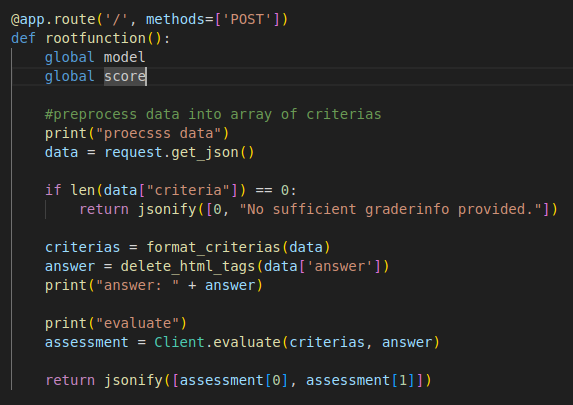
\includegraphics[width=10cm]{rootfunction.png}
\\
\\
Egy request beérkezésekor elsőként  az egy stringként érkező graderinfo-ból kell kicsomagolni a kritériumgondolatokat, illetve a hozzájuk tartozó pontszámokat.
\\
\\
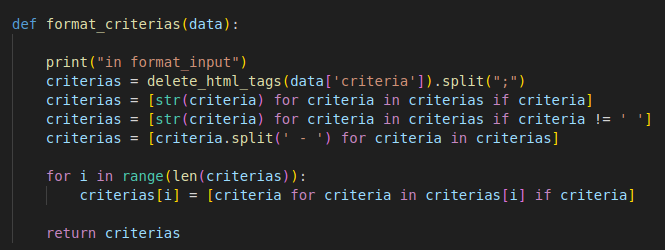
\includegraphics[width=10cm]{format_criteria.png}
\\
\\
Miután a kezünkben vannak a kritériumok és a válasz a megfelelő formátumban, kezdődik a kiértékelés. Ez már modellektől függően változó, de a lényeg, hogy a kritériumok jelenlétét a válaszban egyesével ellenőrizzük. Ha egy kritérium megtalálható a válaszban jár rá a pont, nincs visszajelzés. 
Amennyiben a pont nem jár, egy komment keletkezik.

\subsection{OpenAI}

Az OpenAi-s megoldás esetében az egyes kritériumok ellenőrzése meglehetősn egyszerűen történik:
\\
\\
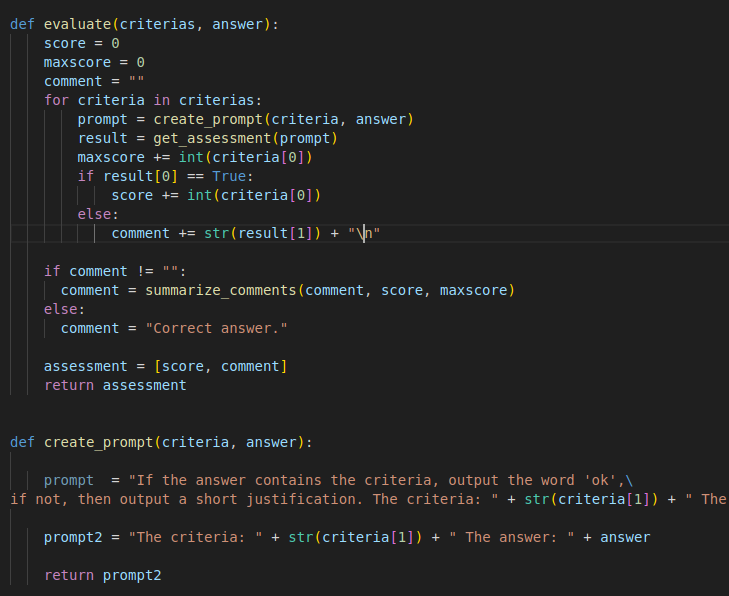
\includegraphics[width=10cm]{openai1.png}
\\
\\
\indent Az evaluate függvényben jól látható, hogy tulajdonképpen egy \"for\" ciklusban egyesével ellenőrizzük a kritériumok jelenlétét.
Létrehozunk egy promptot, ami a gpt-4et felhasználva kideríti a get\_assesment függvényben, hogy jelen van-e a vizsgált gondolat a szövegben.
Amennyiben jelen van, a completion egy egyszerű \"ok\" szó, amennyiben viszont nem, a completion egy magyarázat a pontszám elvételére.
A program az egyes kommenteket egy stringbe konkatenálja, és a kritériumok ellenőrzése után, ha volt hiányzó gondolat meghívja a summarize\_comments
függvényt. Ez egy újabb promptot tartalmaz, amely összefoglalja a kommenteket:
\\
\\
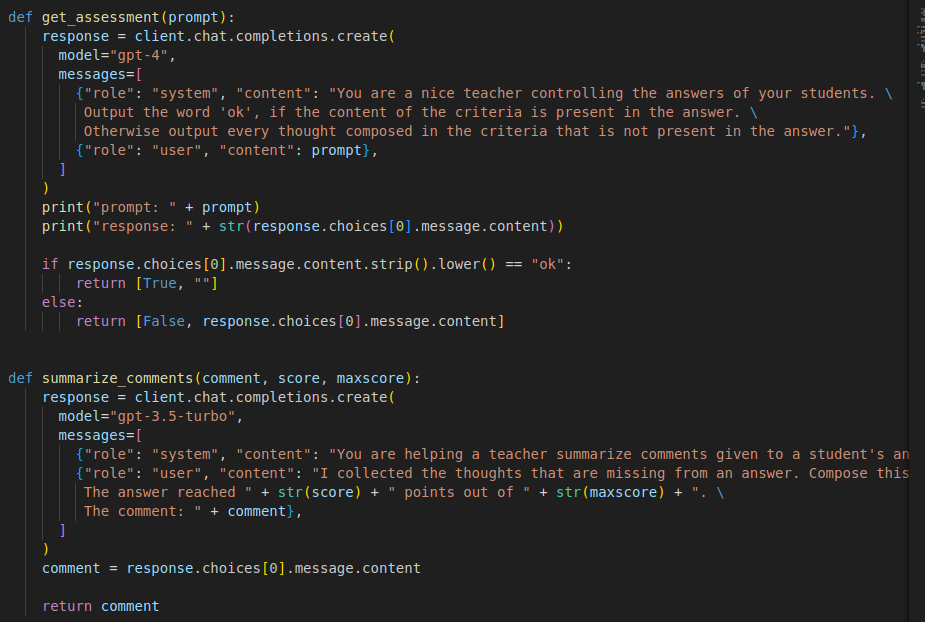
\includegraphics[width=10cm]{sum.png}
\\
\\
\indent Ha ez is meg van, az evaluate függvény visszatér a rootfunctionbe a pontszámmal, és a kommenttel. 

\subsection{Sentencetransformers}

A Sentencetransformers esetében egy picit bonyolultabb a helyzet. Itt direkt módon mi hasonlítjuk össze a kritériumok, és a válasz vektorait. 
Mivel ezek a vektorok fix méretűek bármekkora is a reprezentált szöveg, érdemes még a beágyazás előtt kisebb darabokra darabolni őket. De mi van ha a kritérium két gondolatból áll,
azaz két tagmondatból? Előfordulhat az is, hogy a két gondolat szétszórva helyezkedik el a válaszban. Az imént felsorolt esetek miatt a kritériumokat, és a választ is tagmondatokra bontva ágyaztam be, és így minden egyes 
kritérium darabkáját összehasonlítottam a válasz minden darabjával. Nyilván a kritériumnak minden részének jelen kell lennie a válaszban, ahhoz hogy járjon rá a pont.
Ebben az esetben így néz ki az evaluate függvény:
\\
\\
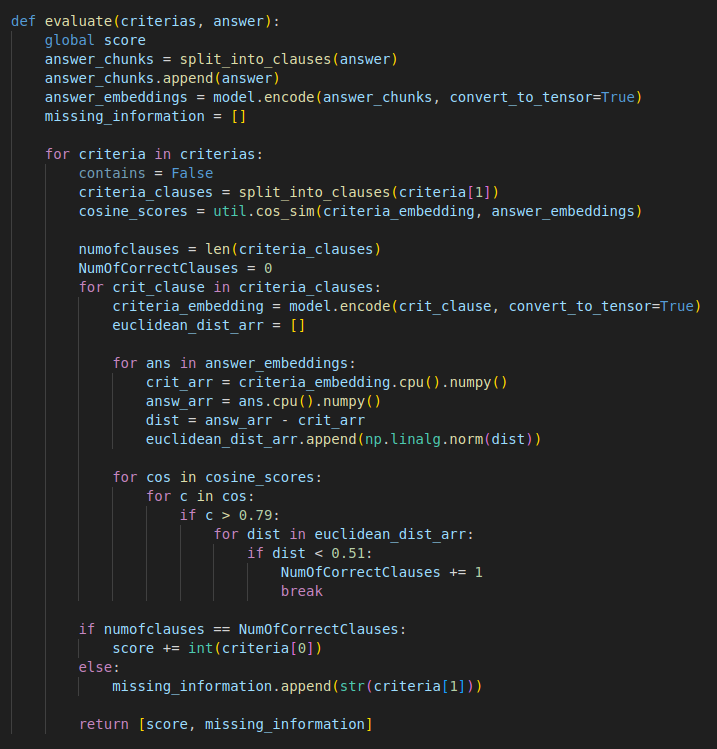
\includegraphics[width=10cm]{eval.png}
\\
\\
\indent Ebben az esetben a komment a hiányzó kritériumok felsorolásából áll.

\section{Moodle integráció}
A moodle integráció egyelőre nincs pluginként megvalósítva, hanem egy moodle core function felüldefiniálásával történik.
Ez a function a \"/moodle/question/behaviour/rendererbase.php\" mappában található. A függvényt a 102. sortól szerkesztettem:
\\
\\
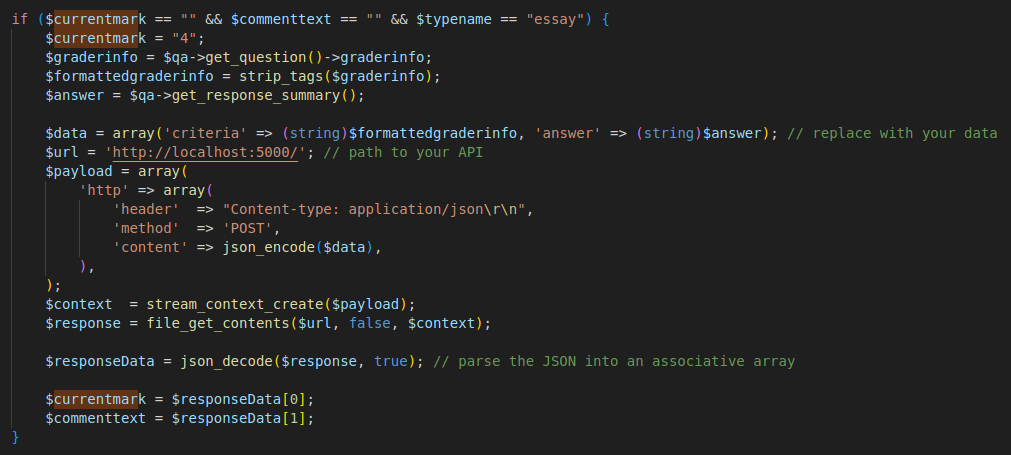
\includegraphics[width=10cm]{moodle.png}
\\
\\
\indent Amennyiben a válasz még nem került értékelésre, a review ablak megnyitásakor a függvény egy kérést intéz a docker konténerben futó szerverhez, amely a válasz, és a graderinfo alapján visszatér a pontszámmal, és a kommenttel.
A mentés gomb megnyomásával a komment és a pontszám elmentődik az adatbázisba, és a következő review ablaknál már ez fog megjelenni, és nem küld új kérést a szervernek.

\section{Haladási napló}

\subsection{Első hét}
Az elmúlt héten leginkáb azzal voltam elfoglalva, hogy a témába beleássam magam. 
Megnéztem a gyorstalpaló kurzus első két heti anyagát, illetve olvasgattam a témában
több cikket is ami ezzel foglalkozik.

Jelenleg még mindig nem egyértelmű számomra, hogy a gyakorlatban hogyan fog megvalósulni a projekt.
Felmerült bennem két kérdés:
\begin{itemize}
  \item Lehetséges, hogy több modell ötvözéséből jön majd létre a végső alkalmazás? (egy kérdés/válasz értelmező + egy pontozó LLM)
  \item Hogyan fog létrejönni az én datasetem a fine-tuninghoz?
\end{itemize}
A project lifecycle-t ha követem a következő feladatok várnak rám:
 
\begin{enumerate}
  \item Use case meghatározása  (Ez elvileg készen van)
  \item Modell kiválasztása  --> Encoder-only? (BERT)
  \item Prompt engineering, fine-tuning, evaluate   + Dataset összeállítása
  \item Alkalmazás integrálása
\end{enumerate}

Jelenleg azt tervezem, hogy 8 hét alatt végzek az LLM-el, és a maradék időben annak
integrálására fogok koncentrálni.
Reményeim szerint a jövőhét folyamán megtalálom a megfelelő transformer architektúrát,
és elkészítem az első prototípust.

Elkezdtem megírni a specifikációmat is, az LLM leírása már fent van a githubon.
Az önlab keretein belül a megbeszélteknek megfelelően elsősorban erre koncetrálnék.

\subsection{Második hét}
Az előző alkalom óta elkezdtem kísérletezgetni LLM-ekkel, megcsináltam több tutorialt is,
szereztem némi gyakorlati tapasztalatot fine-tune-olásban. 

Mivel számomra teljesen új maga a python nyelv is, utána kellett néznem több esetben 
a szintaxisnak, illetve több library működésének: pandas, numpy, datasets, evaluate.

Traineléshez kipróbáltam a tensorflowt, illetve a pytorchot is. Egyelőre a pytorch tűnik számomra szimpatikusabbnak,
mivel lehetőség van nativ tuneolásra.

Megismerkedtem az adatok preprocesszálásához használt eszközökkel, mint a padding, trucation, tokenization, mapping.
Kezd összeállni a kép, hogy hogyan is kell elképzelni egy modell fine-tune-olását, azonban még messze a cél.
Egyre inkább látom, hogy valóban vannak mélységei ennek a témának, és nem olyan egyszerű ez a gyakorlatban, 
mint ahogy azt én az elején elképzeltem. 

Beszéltünk róla az első héten, hogy Szerinted érdemes lenne vscode-ot használni a fejlesztéshez, 
azonban egyelőre még nem találtam meg a megfelelő setupot hozzá.
Probálkoztam az egyik tutorialban említett unweave-vel, mivel jelenleg nem áll rendelkezésemre egyetlen gpu sem, 
azonban ez valamiert nem működött. Így a példa-kódokat egyelőre csak google colabban tudtam futtatni.
Amennyiben Te rendelkezel gyakorlattal az unweave használatában, elfogadnék benne némi segítséget... 
Az egészhez még kicsit hozzátartozik, hogy vasárnap végül elegem lett a windowsból, és azóta az ubuntus közösséget gyarapítom. :)

Ma még utána fogok nézni, hogy az egyes modelleket fine-tuneolás után hogyan lehet lementeni, 
majd egy másik alkalmazásban felhasználni.  

\subsection{Harmadik hét}
Ezen a héten elkezdtem összeállítani a promptok formátumát, amit később a fine-tuneoláshoz használni fogok.
Ehhez elsősorban a chatgpt-vel kísérletezgettem, one-shot után pedig már tök jó eredményeket kaptam.
Csináltam few-shotot is, azzal már az ismeretlen feladatok is egészen helyesen lettek pontozva.

Ezután elkezdtem más modellekkel is kísérletezni huggingfacen:
\begin{itemize}
  \item google/flan-t5-base/xxl \-\-\> a base verzióval nem kaptam eredményeket, xxl-el már volt output, közelítőleg helyes.
  \item bert-base-uncased \/ xlm-roberta-base \/ roberta \-\-\>  volt output, egészen jó. xlm-roberta tud magyarul is.
  \item gpt2 --\> nem volt output
\end{itemize}

Az eddigi próbálkozások alapján a (encoder-only) Bert alapú modellek a legjobbak. Kíváncsi vagyok, ha 
rendelkezem majd nagyobb adathalmazzal melyik hogyan fog teljesíteni. Az eddig használt adatok megtalálhatók githubon 
a data.json fájlban, illetve a átláthatobb formátumban az example fájlokban is.

A mai nap folyamán szeretném még a githubra már feltöltött jegyzetfüzetet befejezni, és legalább a flan-t5-ön lefuttatni a 
traininget. 

Ezen kívül ezen a héten különösebb kérdés nem merült fel bennem, a következő lépések is tiszták számomra. Cél lehet jövőhétig a 
bert típusú, és a flan-t5 modellek tesztelése (), esetleg egy gradio tesztfelület elkészítése is hozzá. Ezzel együtt tovább bővíteném
a datasetet is, első lépésbe angol nyelvű, később akár a xlm-bert model számára magyar nyelvű kérdésekkel is. 

\subsection{Negyedik hét}
Elmaradt

\subsection{Ötödik hét}
Ezen a héten már tényleg sokat kísérletezgettem a modellekkel, első sorban a flan-t5, illetve a bert alapú modellek
fine-tuneolásával.
Jelen állás szerint a modell feladata egyszerűen osztályozni, azaz egy pontszámot adni a válaszra,
a megadott kérdés, illetve pontozási útmutató kontextusában.
\\
\\
\textbf{prompts\_flan\_t5\_base.ipynb}
\\
\\
\indent In this file, I played around with data preprocessing. The tokenize function was completed, which I will use in the future.
In addition to the base model, I also tried the large model, the xl was already too big to download, more precisely it would have taken a very long time.
By the way, the base model gave quite good answers, after full fine-tuning the error function was 49\%.
\\
\\
\textbf{prompts\_bert\_based.ipynb, roberta\_fine\_tune.ipynb}
\\
\\
\indent Then I experimented with the Bert-based models as well. The plain bert didn't work very well,
it didn't even hit that the score should be a digit.
Roberta performed quite well compared to this, I even tried to fine-tune it, but I was not successful:
"TypeError: RobertaModel.forward() got an unexpected keyword argument 'labels'"
After several attempts and error messages, I got here, but I gave up at this point and decided to try fine-tuning the flan-t5 large model
(https://hackernoon.com/fine-tuning-roberta-for-topic-classification)
\\
\\
\textbf{flan\_t5\_large\_peft.ipynb}
\\
\\
\indent In this file, you can find my related attempts, which were also unsuccessful. For some reason,
google colab always decided to crash during training, even if I only tried with the base model.

\subsection{Hatodik hét}

Az előző hét folyamán igyekeztem végre sikeresen peft fine-tuneolni a flan-t5-ös modelleket, ami váratlan módon minden
módosítás nélkül egyből sikerült. Erre nem nagyon találtam magyarázatot.

Ezután sokat játszadoztam a training paraméterekkel, illetve chatgpt-vel felduzzasztottam a data.json fájlt ehhez.
Kis tesztelgetés után arra kellett rájönnöm, hogy nem igazán fejlődik a modell. Akárhogy fine-tuneoltam, annak ellenére, hogy csak
pontoznia kellett a modellnek a válaszokat a "scoring guide" alapján, nem igazán érződött a fejlődés.
Végülis utánanéztem más dataseteknek, mit tudnék a promptomon csiszolni, és így létrejött egy második formátum is. 
Illetve most már próbáltam a megbeszélteknek megfelelően úgy alakítani a promptot, hogy a végeredmény a pontszámon felül egy szöveges értékelést is tartalmazzon.
Na ez az új verzió chatgptve nagyon jól működött, azonban a flan-t5el ismét csak nem jutottam túl sokra.

Végső soron a többi datasetet elnézve felmerült bennem a kérdés, hogy nem túl komplex-e egy ilyen feladat egy flan-t5 számára.
Múlt héten meg ezen a héten elég sokat próbálkoztam vele, és kezd gyanús lenni, hogy érdemes lenne átállni az openAI API-jára.

\subsection{Tizedik hét}

Miután a \textbf{Flan-T5-XL} modelljét nem tudtam fine-tuneolni, az elmúlt két hétben elkezdtem kicsit más irányba tapogatózni.
Jobban beleástam magam a \textbf{LangChain} működésébe, és elkezdett gyanús lenni számomra, hogy valahogy az embeddingek irányába kellene  a későbbiekben továbbhaladnom. Eddig promptokkal próbáltam eldöntetni az LLM-ekkel, hogy egy adott kritérium szerepel-e a válaszokban, azonban találtam modelleket, amik kifejezetten mondatok/szövegek szemantikai összehasonlítására vannak kitalálva.

Így került a kezeim közé a \textbf{SentenceTransformers} framework, annak ``all-mpnet-base-v2'' modellje, amely teljesen szabadon felhasználható, kicsi, gyors, fent van a huggingfacen, és meglehetősen pontosan működik. A \textit{data\_v3}-ban található tesztadatokkal jelenleg 83.3\%-os pontosságot értem el, ez elég jelentős javulás az eddigiekhez képest. A \textit{HF\_Sentencetransformer.ipynb} fájlban találhatóak a próbálkozásaim.

Jelenleg úgy képzelem el az alkalmazást, hogy a tanár által létrehozott tesztfeladatok, illetve a hozzájuk tartozó javítási útmutatók 
elmentődnek valamilyen formátumban a szerveren id-vel, így javításnál könnyedén lekérdezhetők lesznek a kritériumok, nem kell vectore storet használni.

Amivel még nem sokat foglalkoztam az a kódok ellenőrzése. Ennek megoldására is egy ``Sentence similarity'' modellt képzelek el, amelyet már találtam is néhányat, csak a C++ nyelvet ismerőből van hiány. Azonban ha minden igaz ez a szöveges válaszok ellenőrzéséhez elég hasonlóan működhet majd.

Emmellett elvégeztem két gyorstalpaló kurzust a \textbf{moodle academy} oldalán, így plugin fejlesztésben is történtek előrelépések.

\subsection{Tizenegyedik hét}
A héten leginkább a moodle plugin fejlesztésével foglalkoztam, amivel egész jól haladtam, azonban beleütköztem néhány nehézségbe. Jelenleg ott tartok, hogy felhasználóként értem hogyan működnek az egyes quizek, és van egy elképzelésem, hogy hogyan is illeszkedik majd a kész rendszerbe az én pluginom. 

A legjobb megoldásnak az tűnik, ha átírom a quiz activityt, aminek azonban hiányzik a dokumentációja a moodle oldaláról. Ezt még nem tudom pontosan hogyan fogom kikerülni, azonban az egyes APIkkal már sokat kísérleteztem. Alapvetően az elején ijesztőnek tűnt számomra az egész rendszer, és bár még a tényleges kódnak nem láttam neki, a héten nagyon sokat tisztult számomra mit és hogyan kell majd csinálnom.

\subsection{Tizenharmadik hét}
Ezen a héten alapvetően a program moodlebe való integrálásán dolgoztam.
A tanár a zh értékelése során amikor egy válasz kísérlet kommentálására megy, a megjelenő ablakban automatikusan kitöltődik a komment fül
a hiányzó gondolatok megjelölésével, és ez alapján a pontszám is becslésre kerül. Amennyiben a javító a mentés gombra megy, az értékelés mentésre kerül. Ellenkező esetben nem mentődik el semmi, és az ablak újranyitásánál a program ismételten átnézi a választ, és értékel.

A működéshez belenyúltam a php kódba, amely így a review ablak megnyitásánál egy kérést intéz a docker konténerben futó backendhez, amely egy a pontszámot, és a kommentet tartalmazó tömbbel tér vissza. A konténer paraméterként a választ, és az értékelési útmutatót kapja meg, amelyeken koszinuszos összehasonlítást végez a sentencetransformers könyvtár segítségével. Az értékelés pontosságával még nem igazán vagyok elégedett, utolsó héten még legfőbbképpen ezen fogok dolgozni. 

\subsection{Tizennegyedik hét}
Szerdán prezentálok, és szerettem volna előtte még egy utolsó helyzetjelentést küldeni, illetve két kérdést feltenni.

A 13. hét óta készítettem egy másik megoldást gpt használatával is, hogy fel tudjak mutatni egy teljes mértékben késznek mondható megoldást is. Ezt feltöltöttem githubra.

Amivel a legtöbbet próbálkoztam az elmúlt 2 hétben az a moodle plugin elkészítése, de ez sehogy sem akart összejönni... Próbáltam a moodle themekhez hasonlóan overrideolni az eredeti függvényt, de ezt sajnos csak a rendererekkel lehet megtenni, sima mezei core functionnal nem.

Ezen kívül még a sentencetransformerses megoldást csiszolgattam, de még van vele egy kis dolgom holnap.

Továbbá elkészítettem a prezentációmat, ezt mellékletben csatolom. A sentencetransformerses  részen kívül készen van minden. Ha holnap jut rá időd átfutni, azt megköszönöm, de ha nem, az sem baj.

Elkezdtem a mai nap folyamán dokumentációt is írni, mivel egy a tárgyról szóló részletes leírásban megtaláltam, hogy a pótlási hét végéig azt is le kell adni. Azonban én nem emlékszem, hogy a dokumentáció szükségességéről beszéltünk volna, illetve egy szaktársam elmondása szerint neki nem is kellett dokumentációt írni, a konzulenstől függ. Szóval a kérdésem az lenne, hogy az én esetemben ez szükséges-e, vagy elég ha majd csak szakdolgozatként dokumentálom ezt a projektet.


\end{document}